\begin{figure*}[t]
  \centering
  \begin{minipage}[t]{.53\textwidth}
    \vspace{0pt}
    \begin{tikzpicture}
      \node[anchor=south west,inner sep=0] (scene) at (0,0) {%
        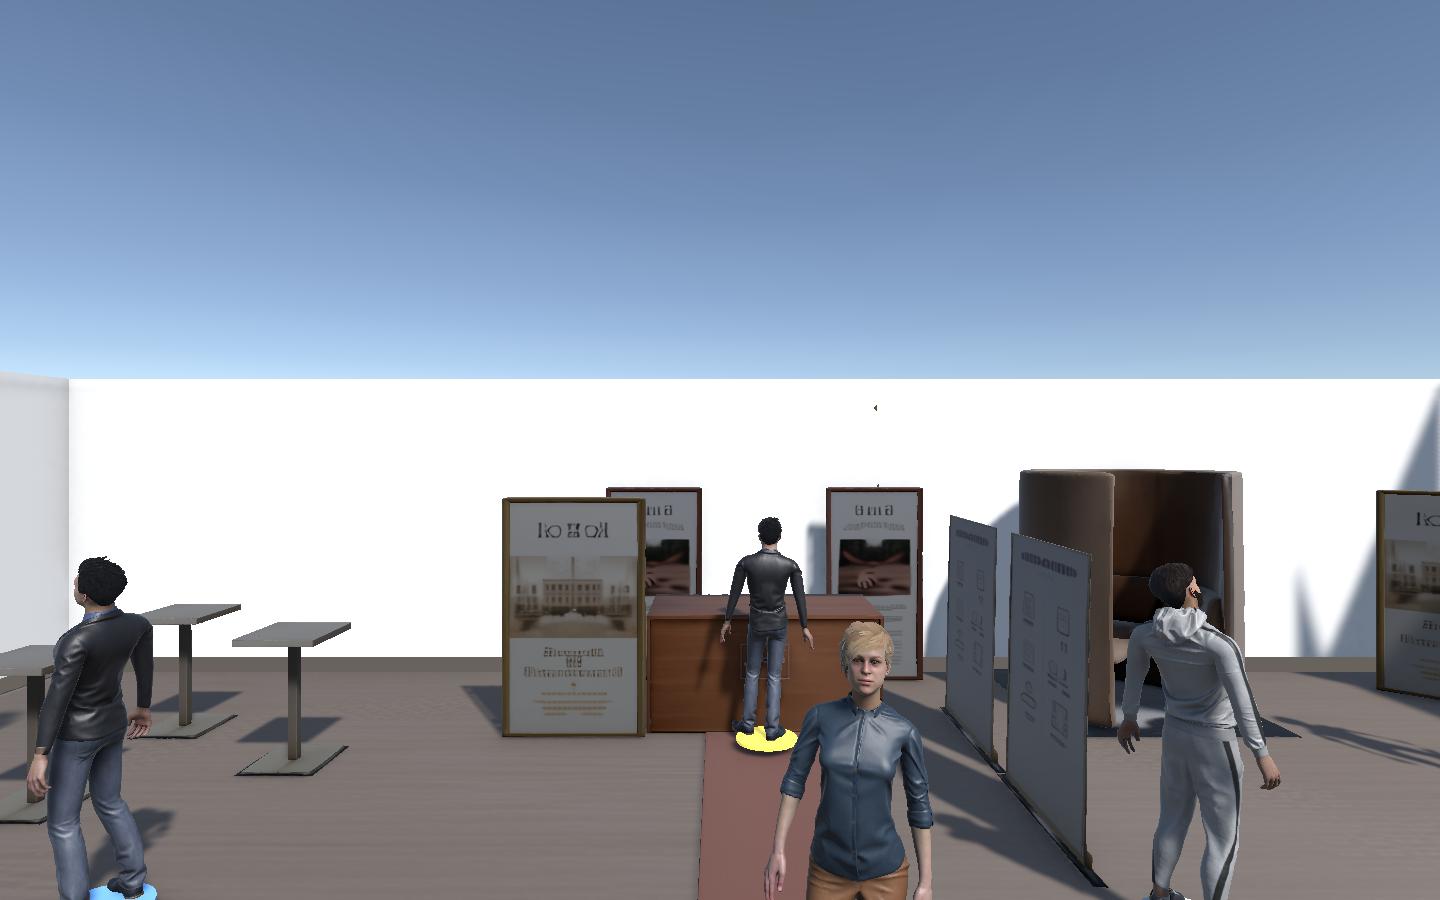
\includegraphics[
          alt={Actual Unity Game view of the Steinpilz exhibition room after
          the model-grounded brand panel selection},
          width=\linewidth
        ]{figures/unity-model-grounded-selection.png}};
      \begin{scope}[x={(scene.south east)},y={(scene.north west)}]
        \draw[cyan!75!black,line width=1.2pt]
          (0.474,0.368) circle[radius=.032];
        \node[
          anchor=west,
          rounded corners=1pt,
          fill=white,
          fill opacity=.94,
          text opacity=1,
          draw=cyan!75!black,
          font=\sffamily\scriptsize,
          align=left
        ] (target-label) at (0.035,0.80)
          {\textbf{Resolved Unity target}\\
           \texttt{brand\_panel3}\\
           \texttt{ENT-ASSET-BRAND\_PANEL3}};
        \draw[-{Latex[length=2mm]},cyan!75!black,line width=.9pt]
          (target-label.east) -- (0.452,0.381);
      \end{scope}
    \end{tikzpicture}

    \centering\footnotesize
    (a) Actual Unity Game view after model loading and target selection.
  \end{minipage}
  \hfill
  \begin{minipage}[t]{.43\textwidth}
    \vspace{0pt}
    \begin{tikzpicture}[
      node distance=2.1mm,
      every node/.style={font=\sffamily\scriptsize},
      tracebox/.style={
        rounded corners=1.5pt,
        draw=black!45,
        fill=blue!5,
        align=left,
        text width=.91\linewidth,
        inner sep=4pt
      },
      rejectbox/.style={
        rounded corners=1.5pt,
        draw=red!65!black,
        fill=red!5,
        align=left,
        text width=.91\linewidth,
        inner sep=4pt
      },
      flow/.style={-{Latex[length=1.8mm]},black!55,line width=.65pt}
    ]
      \node[tracebox] (s1) {\textbf{1. Bind the observation.}
        Collider source \texttt{brand\_panel3} resolves to the exact model
        entity shown at left.};
      \node[tracebox,below=of s1] (s2) {\textbf{2. Resolve responsibility.}
        The asset-level owner is the Reception Agent. From the Lounge Host,
        one declared handoff reaches that owner.};
      \node[tracebox,below=of s2] (s3) {\textbf{3. Select the declared operation.}
        The scenario step uses
        \texttt{ANSWER-ROOM-GROUNDED-QUESTION} with the asset, branding group,
        and entrance zone as targets.};
      \node[tracebox,below=of s3] (s4) {\textbf{4. Re-resolve execution.}
        The pinned binding maps the capability to
        \texttt{BACKEND-CHAT} (\texttt{POST /chat}).};
      \node[tracebox,below=of s4] (s5) {\textbf{5. Return inspectable evidence.}
        Target, provider, capability-use, capability, binding, and action IDs
        are preserved. Contract verdict:
        \texttt{accepted\_with\_evidence}; the grounded-answer assertion remains
        declared rather than semantically judged.};
      \node[rejectbox,below=3.2mm of s5] (reject) {\textbf{Fail-closed contrast.}
        Career Advisor $\rightarrow$ Lounge Host $\rightarrow$ Reception Agent
        needs two handoffs, so the request stops before the response stub and
        does not mutate conversational state.};
      \draw[flow] (s1) -- (s2);
      \draw[flow] (s2) -- (s3);
      \draw[flow] (s3) -- (s4);
      \draw[flow] (s4) -- (s5);
    \end{tikzpicture}

    \centering\footnotesize
    (b) The implemented admission path and its one-hop boundary.
  \end{minipage}
  \caption{Concrete model-grounded interaction in the Steinpilz scene. The
  left image is a reproducible capture from the implemented Unity project; the
  cyan marker and label are paper annotations placed at the collider center
  logged by the capture runner, not additional visitor controls. The right
  side follows the exact success and rejection cases reported in the benchmark.}
  \Description{A two-part figure. On the left, an actual Unity Game view shows
  a virtual exhibition room with embodied agents and display panels. A cyan
  paper annotation marks the selected brand panel and gives its source and
  entity identifiers. On the right, five boxes trace selection, responsibility,
  capability, runtime binding, and returned evidence. A red box contrasts a
  two-handoff route that is rejected before response generation.}
  \label{fig:unity-walkthrough}
\end{figure*}
